\subsection{Überblick}
\label{sec:langmodels}

    In diesem Abschnitt sollen die theoretischen Aspekte der Wortvorhersage erleutert werden. Es handelt sich hier um das Themengebiet des \emph{Natural Language Processing}. In diesem Abschnitt werden dazu ausschließlich Sprachmodelle behandelt. Um Annahmen darüber zu machen, welche Wörter nach einem anderen folgen können, benötigt man zunächst einmal ein Modell der verwendeten Sprache. Im optimalen Fall kann ein \emph{Sprachmodell} eine Sprache und die Beziehung zwischen Wörtern umfassend abbilden. In \autoref{sec:design-learnerPredictor} wird ein \emph{Sprachmodell} als Sammlung von Dateien mit Informationen über einen Text definiert. In diesem Abschnitt geht es um die Bedeutung dieser Informationen.
        
    Eine naheliegende Möglichkeit ein Modell einer Sprache zu generieren ist das Formulieren einer \emph{Grammatik}. Hierbei wird versucht die sytaktischen Regeln einer Sprache zu definieren. Im entworfenen Prototypen spielen solche \emph{Grammatiken} keine Rolle. Darum werden diese nur sehr kurz erklärt.
        
    Ein Beispiel einer einfachen Grammatik ist in \autoref{fig:grammer} zu sehen. \texttt{S -> NP VP} beschreibt, dass ein Satz \texttt{S} aus einem \emph{Noun Phrase} \texttt{NP} und einem \emph{Verb Phrase} \texttt{VP} bestehen kann. Alle weiteren Regeln funktionieren entsprechend. Mit Hilfe einer solchen Grammatik ist es möglich die Funktion eines Wortes innerhalb von einem Satz zu bestimmen. Dieser kann dann, wie in \autoref{fig:parsingTree} zu sehen,  als \emph{tree} dargestellt werden. Im Beispiel gilt es zu beachten, dass \autoref{fig:grammer} nicht alle in \autoref{fig:parsingTree} enthaltenden Worte enthält und somit erst einmal nicht funktionieren würde.
        
    Folgen wir also folgender vereinfachten Regel: Innerhalb eines \emph{Preposition Prase} \texttt{PP} nach einer Preposition \texttt{P} und einem Determinator \texttt{DET} muss immer ein Nomen \texttt{N} kommen. Dann können wir in dem Satzteil \texttt{in the …} aus \autoref{fig:parsingTree} nur noch Nomen als Folgewort vorschlagen.
        
    \begin{figure}[H]
		\centering
        \begin{subfigure}{0.49\textwidth}
			\begin{lstlisting}
S -> NP VP
VP -> V NP | V NP PP
PP -> P NP
V -> "saw" | "ate" | "walked"
NP -> "John" | "Mary" | "Bob" | Det N | Det N PP
Det -> "a" | "an" | "the" | "my"
N -> "man" | "dog" | "cat" | "telescope" | "park"
P -> "in" | "on" | "by" | "with"
    		\end{lstlisting}
            \caption{Einfache Grammatik}
            \label{fig:grammer}
		\end{subfigure}
        \begin{subfigure}{0.49\textwidth}
           	\centering
          	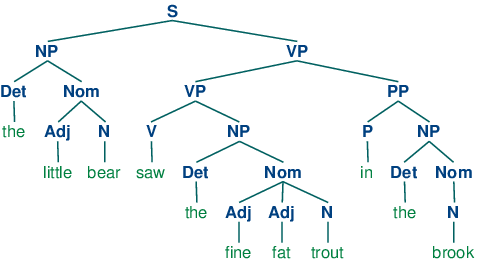
\includegraphics[width=.8\linewidth]{images/grammer.png}
           	\caption{\emph{parsing tree}}
           	\label{fig:parsingTree}
        \end{subfigure}
        \label{fig:grammerWithTree}
        \caption{Beispiel einer einfachen \emph{Grammatik} \parencite[Kapitel 8]{nltk:book}}
        \end{figure}
        \newpage
        
        Allerdings stößt man, wie von \cite[S. 544]{jamia:introduction} im Abschnitt \emph{The limitations of hand-written rules: the rise of statistical NLP} aufgefürht wird, mit solchen \emph{Grammatiken} an Grenzen. In dem Artikel werden zwei Probleme solcher \emph{Grammatiken} beschrieben.
    
    	Zum einen beschreiben diese in erster Linie Syntax und nicht die Semantik eines Satzes. Dies kann laut \cite{jamia:introduction} zwar durch Erweitern der Regeln gelöst werden. Sie Nutzen hier das Beispiel, dass das Verb \texttt{essen} nur für bestimmte \emph{essbare} Nomen gültig gemacht werden kann. Weißen aber darauf hin, dass so die Regeln viel zu komplex und unüberschaubar würden.
        
        Als zweites Problem führen sie an das solche \emph{Grammatiken} mit Sätzen, die zwar von Menschen verstanden werden aber nicht unbedingt grammatischen Regeln folgen, nicht umgehen können.
        
        \cite{jamia:introduction} beziehen sich bei Ihren Überlegungen, auch wenn sie Anwendungsbeispiele aus der Medizin nutzen, auf \emph{Natural Language Processing} im Allgemeinen. Hier soll versucht werden diese Formulierungen bezüglich der Wortvorhersage zu verwenden.
        
        Aufgrund der genannten Probleme gab es, wie \cite{jamia:introduction} auf Seite 545 schließen, in den 1980ern eine Wende hin zu \emph{statistischem Natural Languge Processing}. Sie erklären \enquote{[\dots]fewer, broader rules replace numerous detailed rules, with statistical-frequency information looked up to disambiguate.} Übersetzt meinen sie also, dass weniger aber weiter gefasste Regeln in Kombination mit statistischen Frequenzen detaillierte Regeln ersetzen. Ein Beispiel für solche statistische Modelle sind die in \autoref{sec:n-gramms} erklärten \emph{N-gramms}.
        
        Ein statistisches Modell basiert immer auf Wahrscheinlichkeiten. Im gleichen Abschnitt beschreiben \cite{jamia:introduction} auch, dass diese Wahrscheinlichkeiten abhängig sind von dem Text aus welchem die Statistiken generiert werden. So liefert vereinfacht Formuliert eine auf Prosa Texten gelernte Statistik keine guten Ergebnisse auf Wissenschaftliche Texte.
